\documentclass{swfuthesise}

%\usepackage{wx672nerd}
\usepackage{lipsum}

%\includeonly{chapters/ch2-quick}

\addbibresource{example.bib}

\swfusetup{
  Title        ={How to mess up everything in Hogwarts},
  Author       ={Harry Potter}, % 作者姓名
  Signature    ={\includegraphics[width=6em]{signature.pdf}}, % 作者签名(用于原创声明页)
  ID           ={201801888}, % 学号
  Year         ={2021},
  Month        ={December},
  Date         ={3},
  % Major        ={Computer Science},%
  Advisor      ={Prof. Albus Dumbledore}, %第一指导教师,第二指导教师
  % Reviewer ={Name (Title)}, % 评阅人
}

\begin{document}

\maketitle
%\frontmatter

\begin{abstract}
  \lipsum[1-3]

  \begin{keyword}
    Black magic; Dark art defence; Spells development; Muggle study;
  \end{keyword}
\end{abstract}

\tableofcontents % 目录
% \clearpage
% \listoffigures % 图片目录,可以没有
% \clearpage
% \listoftables  % 表格目录,可以没有

%\mainmatter

\chapter{Introduction to Hogwarts}
\label{cha:intr-hogw}

\section{History}
\label{sec:history}

Founded in the 10th century by Godric Gryffindor, Rowena Ravenclaw, Helga Hufflepuff and
Salazar Slytherin, Hogwarts was established in the Highlands of Scotland to educate young
wizards and witches as well as to keep students safe from muggle
persecution.\cite{harrypotter} Theory has it that Rowena Ravenclaw came up with the name
of Hogwarts after dreaming of a warty hog that led her to a cliff by a lake. Since then,
Hogwarts educated most wizarding children in the United Kingdom and its surrounding areas,
keeping its location hidden from other wizarding schools and
muggles.\cite{nla.cat-vn992642,nla.cat-vn7290756} Fig.~\ref{fig:hogwarts} shows the main building of Hogwarts school.


\begin{figure}
  \centering%
  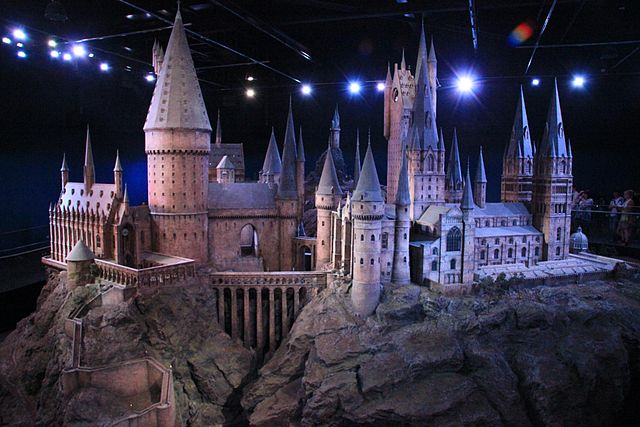
\includegraphics[width=.4\textwidth]{Hogwarts.jpg}
  \caption{Studio model of Hogwarts at Leavesden Studios\label{fig:hogwarts}}
\end{figure}

\lipsum[3-4]

\section{Good guys and bad guys}

\lipsum[][2]. Table~\ref{tab:hp} lists a good guy and a bad guy of Hogwarts. 

\begin{center}\singlespacing
  \captionof{table}{An example table\label{tab:hp}}
  \begin{tabular}{lll}
    \toprule
    Name&School&Brief Info\\\midrule
    Harry Potter&Gryffindor&Good\\
    Draco Malfoy&Slytherin&Bad\\\bottomrule
  \end{tabular}      
\end{center}

\lipsum[7-8]

\chapter{The fundamental principle of breaking bad}

\lipsum[150]

\section{The general rules}

\lipsum[16-18]

\section{Despicable me}

\lipsum[19-20]

\subsection{More than mess up}

\lipsum[21-23]

\chapter{General Procedure of dark art development}
\label{cha:gener-proc-spells}

\lipsum[31] Figure~\ref{fig:workflow} shows the general workflow of the system.

\begin{figure}[!ht]
  \centering
  \begin{minipage}{.8\linewidth}
\begin{verbatim}
┌───────┐  ┌─────┐  still  ┌─────┐  ┌─────┐  ┌────┐
│Brewing│  │Drink│  alive? │Mount│  │Speak│  │Take│
│potion ├─>│ it  ├─> <> ──>│broom├─>│spell├─>│off │
└───────┘  └─────┘         └─────┘  └─────┘  └────┘ 
\end{verbatim}
  \end{minipage}
  \caption{General work flow}
  \label{fig:workflow}
\end{figure}

\section{Top level design}

\lipsum[32-34]

\section{System modules design}

The main function modules in this systems are:
\begin{itemize}
\item Spells generation
\item Potions brewing
\item Broom control
\end{itemize}

\subsection{Spells generation}
\lipsum[35-36]

\subsection{Potions brewing}
\lipsum[37-38]

\subsection{Broom control}
\lipsum[39-40]

\chapter{Tests and conclusions}

\section{System tests}

\subsection{General test cases}

\begin{description}
\item[Case 1] \lipsum[37]
\item[Case 2] \lipsum[38]
\item[Case 3] \lipsum[39]
\end{description}

\subsection{Corner cases}

\begin{description}
\item[Case 1] \lipsum[40]
\item[Case 2] \lipsum[41]
\item[Case 3] \lipsum[42]
\end{description}

\section{Conclusions}

\lipsum[43-44]

\appendix % 参考文献、指导教师简介、鸣谢、附录

\makebib % 参考文献

\begin{advisorInfo} % 指导教师简介
  
  Prof. Albus Percival Wulfric Brian Dumbledore is a fictional character in
  J. K. Rowling's Harry Potter series. For most of the series, he is the headmaster of the
  wizarding school Hogwarts. As part of his backstory, it is revealed that he is the
  founder and leader of the Order of the Phoenix, an organisation dedicated to fighting
  Lord Voldemort, the main antagonist of the series.

  Dumbledore was portrayed by Richard Harris in the film adaptations of Harry Potter and
  the Philosopher's Stone and Harry Potter and the Chamber of Secrets. After Harris'
  death, Michael Gambon portrayed Dumbledore for all of the remaining Harry Potter
  films. Jude Law portrayed Dumbledore as a young man in the prequel film Fantastic
  Beasts: The Crimes of Grindelwald.

  Rowling stated she chose the name Dumbledore, which is a dialectal word for "bumblebee",
  because of Dumbledore's love of music: she imagined him walking around "humming to
  himself a lot".

\end{advisorInfo}

\begin{acknowledgment} % 致谢
  Thank God, I've done it!
\end{acknowledgment}

%%%%% 附录章节
\singlespacing

\chapter{Not mandatory}

If you want to include long code listings in your thesis, put it here.

\section{C program example}
\label{sec:c-example}

\lipsum[50]

\begin{ccode}
#include<stdio.h>

int main(void)
{
  printf("Hello, world!\n");
}
\end{ccode}

\section{Shell script example}
\label{sec:shell-script-example}

\lipsum[51]

\begin{shellcode}
  #!/bin/bash

  echo 'Hello, world!'
\end{shellcode}

\end{document}
%%% Local Variables:
%%% mode: latex
%%% TeX-master: t
%%% End:
